\paragraph*{3.3} 因为 $f'(x)=1-\dfrac{2}{1+x^2}$, 解得驻点为 $x=\pm 1$. 又 $f''(x)=\dfrac{4x}{\left(1+x^2\right)^2}$, 拐点为 $x=0$.

故
\begin{center}
\begin{tabular}{c|c|c|c|c|c|c|c}
\hline
$x$   & $(-\infty,-1)$ & $-1$ & $(-1,0)$       & $0$ & $(0,1)$         & $1$ & $(1,+\infty)$ \\ \hline
$f'$  & $+$            & $0$  & $-$            & $-$ & $-$             & $0$ & $+$           \\ \hline
$f''$ & $-$            & $-$  & $-$            & $0$ & $+$             & $+$ & $+$           \\ \hline
$f$   & $\uparrow$ 下凹  & 极大   & $\downarrow$ 下凹 & 拐点  & $\downarrow$ 上凹 & 极小  & $\uparrow$ 上凹 \\ \hline
\end{tabular}
\end{center}

$f$ 的单增区间为 $(-\infty,-1)\cup(1,+\infty)$, 单减区间为 $(-1,1)$.
\[
	f_{\max}=f(-1)=\dfrac{\pi}{2}-1,f_{\min}=f(1)=1-\dfrac{\pi}{2}
\]

$f$ 的图像在 $(-\infty,0)$ 下凹, 在 $(0,+\infty)$ 上凹, $(0,0)$ 是拐点.

渐近线: $x\to+\infty$ 方向为 $y=x-\pi$, $x\to-\infty$ 方向为 $y=x+\pi$. 

\begin{figure}[h]
	\centering
		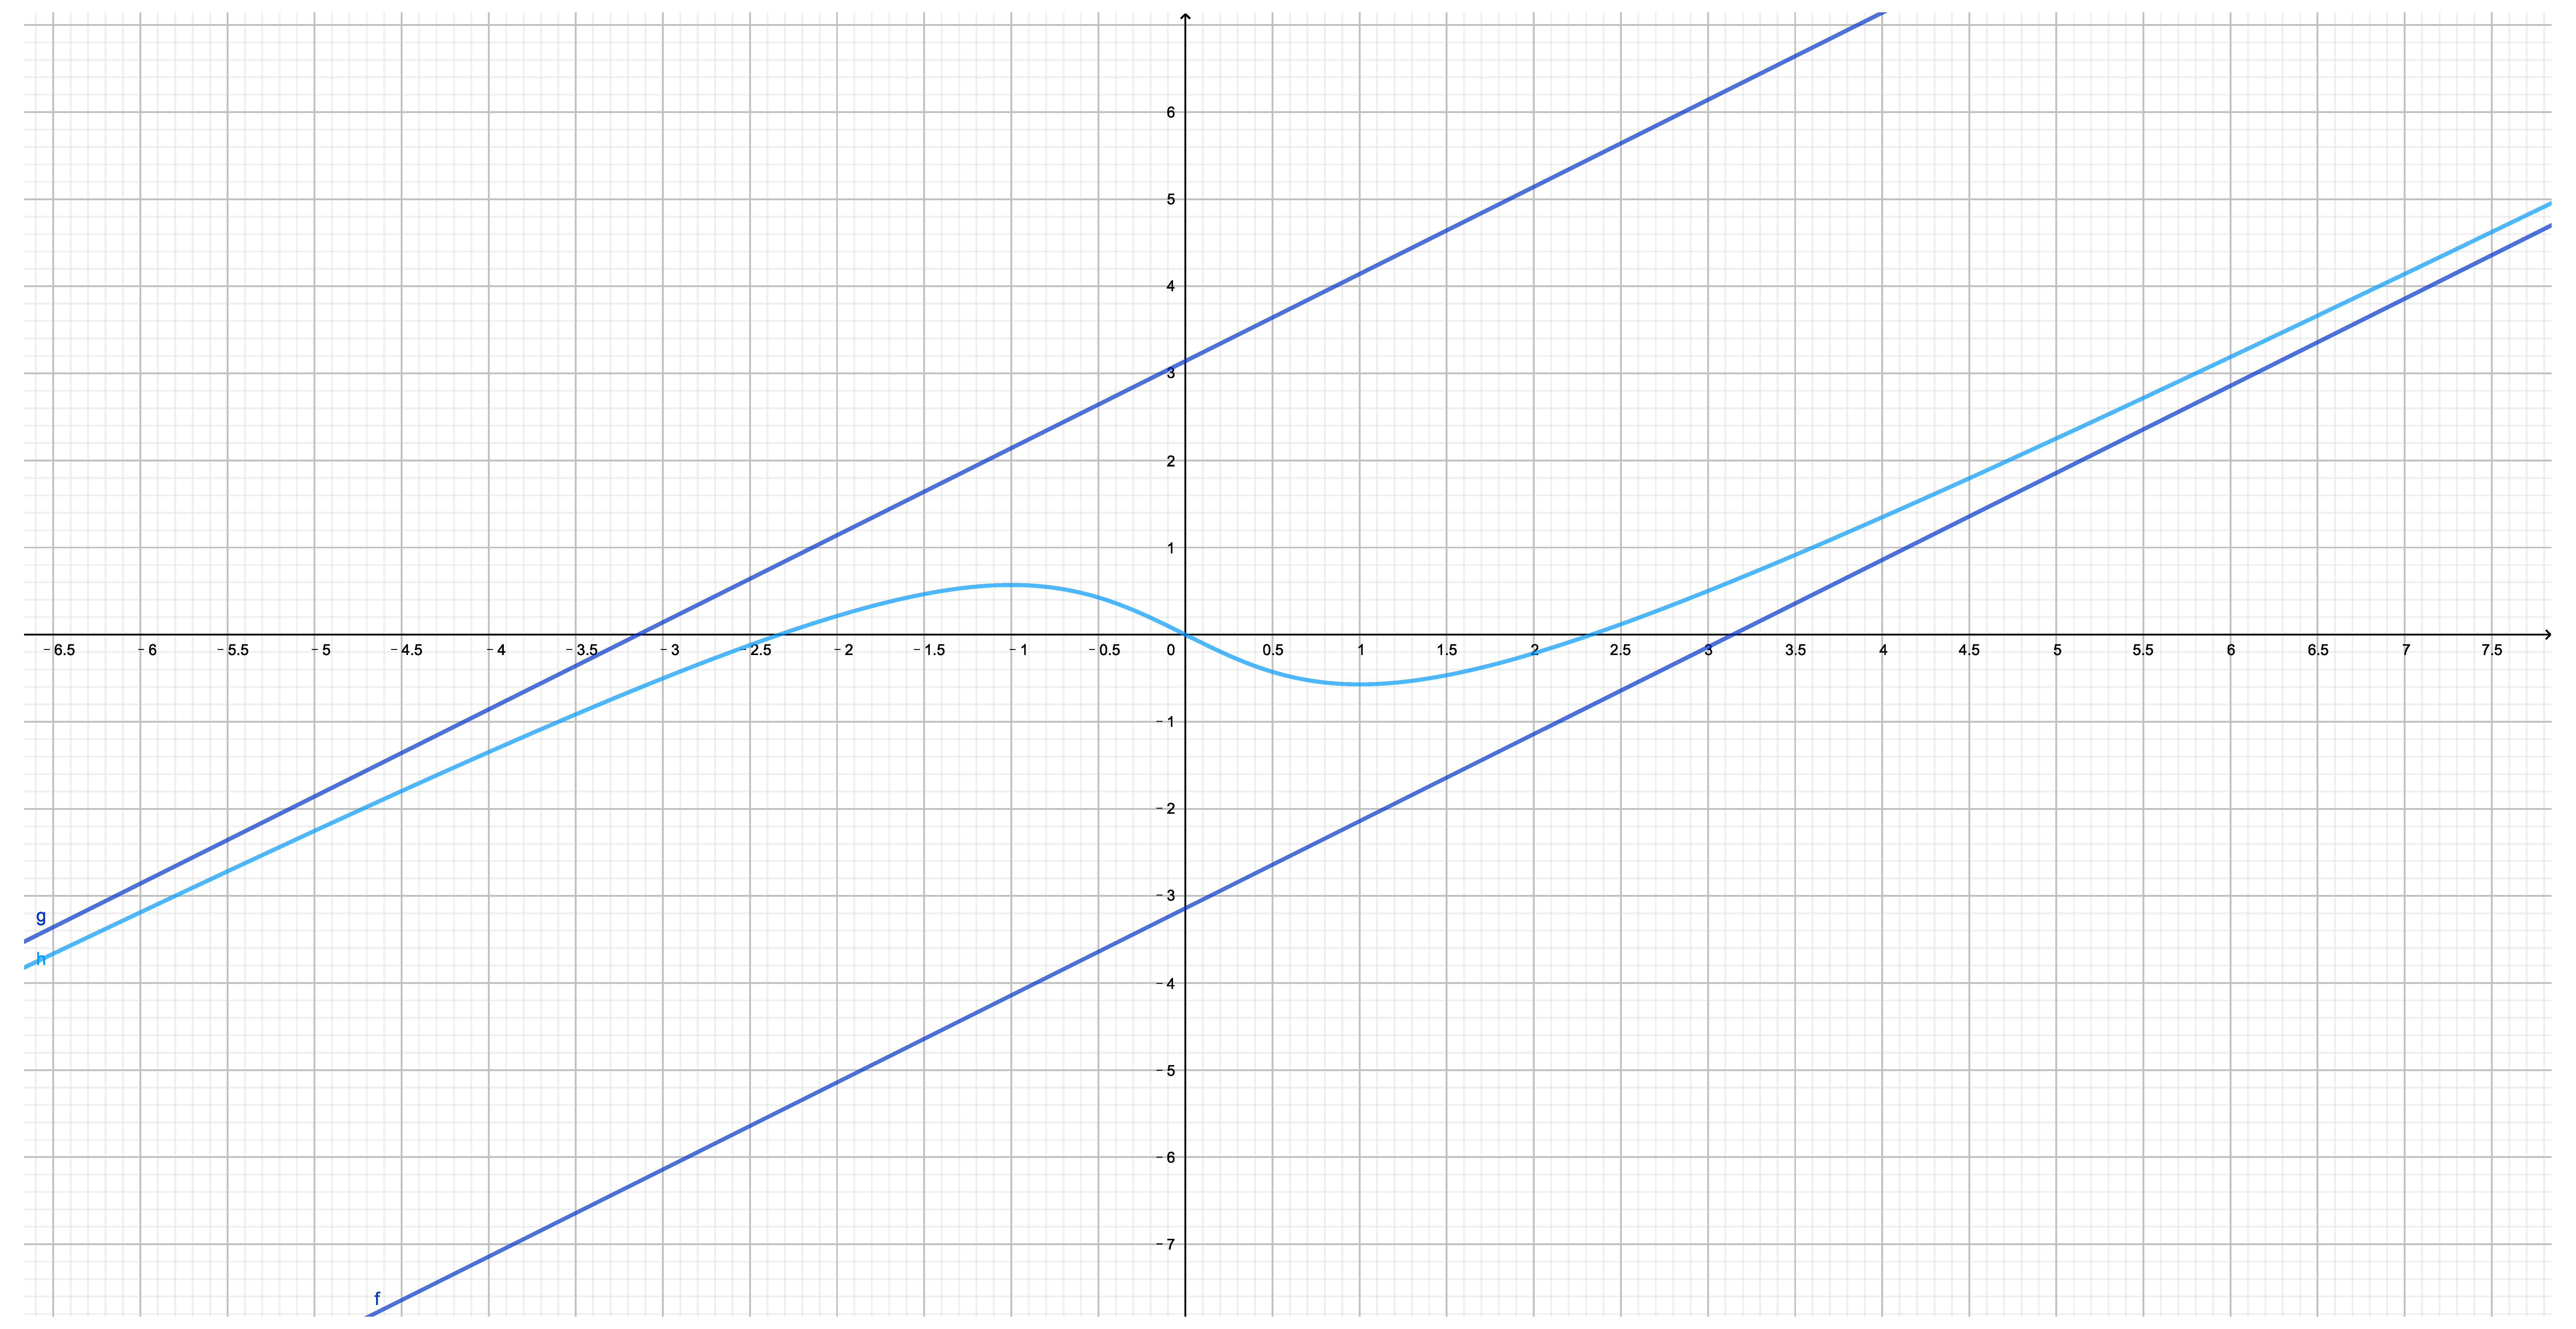
\includegraphics[scale = 0.1]{figure_3.3.pdf}
\end{figure}